\section{Electronic energy calculations}
The Schrödinger equation \ref{schrondinger} revolutionized our comprehension of atomic structures. In this equation, $i$ represents the imaginary unit, introducing a crucial imaginary component for precise quantum treatment. The symbol $\hbar$, the reduced Planck constant, scales the quantum nature of the system. The term $\frac{\partial \psi}{\partial t}$ signifies the rate of change of the wave function ($\psi$) with respect to time, capturing the dynamic evolution of the quantum system. The operator $\hat{H}$ denotes the Hamiltonian, defining the total energy of the system, and the equation asserts that the time rate of change of the wave function is proportional to the application of the Hamiltonian operator on the wave function. Finally, $\psi$ itself represents the quantum state of the system. Therefore, these elements elegantly describe the intricate interplay between a system's evolving quantum state and its underlying energy dynamics. Published in Erwin Schrödinger's crucial work in 1926, this expression provided a mathematical framework for describing the wave-like behavior of quantum mechanical systems, seen in experiments but not well described by any theory at that moment. It introduced the concept of wave functions, which describe the probability of finding a particle at a particular location and time. It goes as follows \cite{SchEq}:

\begin{equation}
\label{schrondinger}
i\hbar \frac{\partial \psi}{\partial t} = \hat{H} \psi
\end{equation}

It has been used to explain a wide range of phenomena in quantum mechanics, including the behavior of atoms and molecules, the properties of materials, and the behavior of subatomic particles. An interesting application of the Schrödinger equation is that it can be used to calculate the electronic structure of various materials, from atoms to solids \cite{SchEq}.

For instance, Figure \ref{e_h} shows this result for the hydrogen atom. It can be noticed that the value of $-13.6eV$ agrees with the experimental values of the ionization energy.
\begin{figure}[!ht]
        \centering
        \includesvg[width=10cm,height=9cm]{images/hydrogen_levels.svg}
        \caption{Energy Levels of the Hydrogen Atom}
        \label{e_h}
\end{figure}

However, even though this equation works well for the Hydrogen atom, finding a formula for atoms with more than one electron is not possible. The reason for this is that when we look at a system with more than two electrons, we can't separate the variables in the equation because of the term that accounts for the interaction between the electrons ($V_{ee}$).

\section{Density Functional Theory}
In this scenario arises the density functional theory  \cite{PhysRev.136.B864}, a brilliant method that seeks to compute all observables as functionals of the electron density. This perspective change made the calculations easier since the electron density is simpler to manipulate than the wave function. This technique is quite popular in materials science because it offers a good balance between accuracy and computational cost.

Nonetheless, in order to trust the obtained results, it is necessary to prove that there is a bijective equivalence between the wave function and the electron density. This crucial paper was accomplished in 1964 by Kohn and Hohenberg\cite{PhysRev.136.B864}, giving rise to what is widely recognized as the Hohenberg-Kohn theorem.

\subsection{Hohenberg-Kohn Theorem}
The Hohenberg-Kohn theorem \cite{PhysRev.136.B864} is a fundamental result in density functional theory that establishes a unique correspondence between an external potential $V_{ext}$ and the electron density of a physical system $\eta (\textbf{R})$. 

This principle is a powerful tool for physical calculations since the wave function can be replaced by the electron density in applying the variational principle, providing a viable way to calculate observables in the ground state.

Finally, one of the main conclusions that this theorem allows us to reach is that we can create auxiliary systems. As long as they contain the same external potential, they must present the same electronic density and, consequently, will exhibit the same properties calculated from the observables.

\subsection{The Total Energy Functional}
Considering the equivalence relation between the electronic density and the wave function in the Hohenberg-Kohn theorem, it is extremely important to study the energy functional, as it plays a central role in future results. One can write the energy functional in terms of the kinetic energy $T$, the electron-electron interaction $V_{ee}$ and the external potential $V_{ext}$:

\begin{equation}
  E[\eta] = \langle \psi | \hat{H} | \psi \rangle = \langle \psi | \hat{T} + \hat{V_{ee}} + V_{ext}  | \psi \rangle = T[\eta] + V_{ee}[\eta] + V_{ext}[\eta]
\end{equation}

In the expression above, the external potential is a one-body operator, allowing its functional to be written as $\int V_{ext}(\textbf{R}) \cdot \eta (\textbf{R}) d\textbf{R}$. However, the kinetic energy and electron-electron interaction operators are unknown, which is why their sum is known as the Hohenberg-Kohn functional.

\begin{equation}
    HK[\eta] = T[\eta] + V_{ee}[\eta]
\end{equation}

The Hohenberg-Kohn functional is the missing piece to obtain an exact expression of the energy functional. In fact, the research for the exact expression of this functional has been an object of interest in several  fronts. Recently, researchers have been approaching the problem in innovative ways, such as using Machine Learning techniques to approximate $HK$ functional\cite{PhysRevLett.125.076402}.

In order to approximate the value of the functional of energy, the Hartree functional can be used as a possible alternative.

\begin{equation}
E_{H}[\eta] = \frac{1}{2}\int\int \frac{\eta(\mathbf{\textbf{R}})\eta(\mathbf{\textbf{R}}')}{|\mathbf{\textbf{R}}-\mathbf{\textbf{R}}'|} \mathrm{d}\mathbf{\textbf{R}}\mathrm{d}\mathbf{\textbf{R}}'
\end{equation}
So, the resulting functional would be:

\begin{equation}
E[\eta] = E_{H}[\eta] + E_{xc}[\eta]
\end{equation}

Where $E_{xc}[\eta]$ is the exchange-correlation term that represents the quantum interactions of the electron with itself, which cannot be described through classical electrostatics.

\subsection{Kohn-Sham Equations}
Thus, considering one of the consequences of the Hohenberg-Kohn theorem regarding auxiliary systems and based on the results of the energy functional, Walter Kohn and Lu Sham published an article in 1965 \cite{PhysRev.140.A1133}. The main idea was the construction of an auxiliary system in which particles do not interact. In this system, electrons move at an effective potential $V_{eff}$ that depends on the electron density of the system. The electron density is determined by the wave functions in the auxiliary system, which are represented below:

\begin{equation}
    \left[-\frac{1}{2}\nabla^{2} + V_{eff}(\textbf{R})\right ] \psi_{i}(\textbf{R}) = \lambda _{i} \psi_{i}(\textbf{R})
\end{equation}
\begin{equation}
    n (r) = \sum _{i} ^{N} |\psi_{i}(\textbf{R})| `^{2}
\end{equation}
where $N$ represents the number of states occupied by the electrons.

Considering the existence of an auxiliary system, the objective is to find the wave functions that describe it. For this purpose, the variational principle is used, which establishes that the chosen wave functions are those that minimize the energy functional. The resulting equations are the following:
\begin{equation}
    \frac{\delta E[\eta]}{\delta \psi _{i}(\textbf{R})} = 0
\end{equation}
Assuming that the wave functions are normalized, the Lagrange multiplier method is used to find a solution.
\begin{equation}
    \frac{\delta E[\eta] -\lambda _{i}(\int \psi _{i} (\textbf{R}) ^{*} \cdot \psi _{i} (\textbf{R})d\textbf{R} -1 ) }{ \delta \psi _{i}(\textbf{R})} = 0
\end{equation}
Expanding the previously mentioned equation, the following result was obtained:

\begin{equation}
\left[-\frac{1}{2}\nabla^2 + V_{ext}(\mathbf{R}) + \int \frac{\eta (\mathbf{R}^{'})}{| \mathbf{R} - \mathbf{R}^{'}|} + \frac{\delta E_{xc}[\eta]}{\delta \eta (\mathbf{R})} \right]\psi_i (\mathbf{R}) = \lambda_i\psi_i(\mathbf{R})
\end{equation}

where $\int \frac{\eta (\mathbf{R}^{'})}{|\mathbf{R} - \mathbf{R}^{'}|} $ is the Hartree potential $V_{H }$ and
$\frac{\delta E_{xc}[\eta]}{\delta \eta (\mathbf{R})} $ is known as the exchange-correlation potential. Then, the equation can be rewritten as follows:

 \begin{equation}
 \label{kohn_sham_eq}
\left[-\frac{1}{2}\nabla^2 + V_{ext}(\mathbf{R}) + V_{H}[\eta,\mathbf{R}] + V_{xc}[\eta,\mathbf{R}] \right]\psi_i(\mathbf{R}) = \lambda_i\psi_i(\mathbf{R})
\end{equation}

Thus, the equation \ref{kohn_sham_eq} demonstrates a proposal for an auxiliary system of non-interacting particles exposed to an effective potential $V_{eff} = V_{ext}(\mathbf{R}) + V_{H}[\eta,\mathbf{R}] + V_{xc}[\eta,\mathbf{R}] $. The \ref{kohn_sham_eq} equation is known as the Kohn-Sham equation.

Finally, it is clear that the \ref{kohn_sham_eq} equation plays a key role in the advancement of materials science, as it allows a self-consistent and computationally efficient resolution of the problem. The self-consistent flow is described by Figure \ref{ks_fc}.

\begin{figure}[!ht]
        \centering
        \includesvg{images/ks_eq.svg}
        \caption{Simplified Flow Chart for Kohn-Sham Equations.}
        \label{ks_fc}
\end{figure}

\subsection{DFT results}
DFT has shown remarkable success in accurately predicting the precise positions of atoms within a spatial structure, achieving an impressive 1\% to 2\% accuracy \cite{DFTCoursera}. However, its performance is not as reliable when it comes to calculating properties dependent on excited states. In such cases, the method tends to underestimate certain characteristics, such as the band gap, by approximately 40\% \cite{PhysRevLett.51.1884}. This discrepancy is readily evident in Table \ref{tab:bandgaps}.

\begin{table}[htbp]
\centering

\caption{Comparison of DFT calculated band gaps with experimental band gaps \cite{PhysRevB.78.125116}}
\begin{tabular}{ c c c}
\hline
\hline
Material & LDA  calculated band gap (eV) & Experimental band gap (eV) \\ \hline
Si & 0.51  & 1.17 \\ 
GaN & 1.95 & 3.507 \\ 
GaAs & 0.41 & 1.519 \\
\hline
\hline
\end{tabular}
\label{tab:bandgaps}
\end{table}

\section{Janak's Theorem and Slater's Technique}
To grasp the calculation of the band gap for complex systems, it is essential to first comprehend the concept itself and how this value is determined within the DFT framework.
\subsection{Band Gap}
The concept of the fundamental band gap \ref{bg} is defined as the energy difference between the highest occupied state and the lowest unoccupied state. Mathematically, it can be expressed as the energy necessary for electron removal from the system subtracted from the energy necessary for electron addition to the same system. These two values are commonly referred to as ionization energy (I) \ref{ie} and electron affinity (EA)  \ref{ae}\cite{DFTCoursera}.
\begin{equation}
\label{ie}
I =  E_{N-1} - E_{N}
\end{equation}

\begin{equation}
\label{ae}
EA =  E_{N} - E_{N+1}
\end{equation}

\begin{equation}
\label{bg}
    E_{g} = I - EA
\end{equation}

%\begin{figure}[!ht]
%        \centering
%        \includegraphics[width=10cm,height=9cm]{images/bs_si.png}
%        \caption{Band structure of Silicon \cite{SiBandStructure}.}
%        \label{bs_si}
%\end{figure}

This property is worth researching because it determines the electrical and optical properties of a material. Materials with large band gaps are typically classified as insulators, while materials with smaller band gaps are typically semiconductors or conductors.
%https://commons.wikimedia.org/wiki/File:Band_structure_Si_schematic.svg
% https://journals.aps.org/prb/abstract/10.1103/PhysRevB.10.5095


\subsection{Janak's Theorem}
Since one has an established definition of the band gap, it is crucial to explore the connection between the energy of a system and the number of electrons it contains, denoted by $N$. Janak's theorem \cite{PhysRevB.18.7165}  aims to establish this relationship and is described by equation \ref{jt}, where the change in energy with respect to electron occupation at a specific level $\alpha$ ($f_{\alpha}$) is equivalent to the eigenvalue of the Kohn-Sham equation at that level, denoted as $\varepsilon_{\alpha}(f_{\alpha})$. A schematic illustration of this system can be seen in figure \ref{occ}.
\begin{equation}
\label{jt}
    \frac{ \partial E}{ \partial  f_{ \alpha } } = \varepsilon  _{ \alpha } ( f_{ \alpha } )  
\end{equation}

\begin{figure}[!ht]
        \centering
        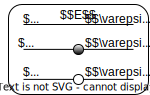
\includegraphics[width=10cm,height=6cm]{images/occupation.png}
        \caption{Schematic representation of occupied levels in a system.}
        \label{occ}
\end{figure}
By assigning the values of -1 to occupied levels and 0 to unoccupied levels, and appropriately developing equation \ref{jt}, an intriguing relationship emerges between the ionization energy and the eigenvalues of the Kohn-Sham equation. This relationship can be expressed by equation \ref{iejt}.

\begin{equation}
\label{iejt}
    I = \int _{0} ^{-1} \varepsilon (f_{\alpha}) d f_{\alpha} 
\end{equation}

Consequently, the ionization energy is determined by integrating the eigenvalues associated with the occupation. Since the electron self-energy introduces linearity into this relationship, it follows that the ionization energy corresponds to the eigenvalue of the last level with half occupation. This concept is captured by equation \ref{jcf}.

\begin{equation}
\label{jcf}
    I = \varepsilon (-\frac{1}{2})
\end{equation}

\subsection{Slater's Technique}
The aforementioned result holds extreme importance and formalizes Slater's technique \cite{PhysRevB.5.844}\cite{SLATER19721}. This method involves removing half an electron from the highest occupied level of an atom and calculating its ionization energy. Notably, as observed in Table \ref{tab:sr}, this approach yields remarkably accurate results that closely align with experimental values.
\begin{table}[htbp]
\centering

\caption{The first ionization energy obtained using the Slater technique can be compared with experimental values\cite{PhysRevB.78.125116}}
\begin{tabular}{ c c c}
\hline
\hline
 & \multicolumn{2}{c}{First IP} \\
Atom & Calc.  & Expt. \\ \hline
C  & 11.60   & 11.26 \\ 
N  & 14.81  & 14.53 \\ 
O  & 13.89  & 13.62 \\
Al  & 5.94   & 5.99 \\ 
Si  & 8.19   & 8.15 \\ 
P  & 10.44  & 10.49 \\
S  & 10.57   & 10.36 \\ 
Zn  & 9.70  & 9.39 \\ 
Ga  & 6.00  & 6.00 \\
Ge  & 7.99   & 7.90 \\ 
As  & 9.90  & 9.81 \\ 
In  & 5.73  & 5.78 \\
\hline
\hline
\end{tabular}
\label{tab:sr}
\end{table}



\subsection{Slater's Technique applied on solids}

While Slater's technique yields remarkable results for atoms, it cannot be directly applied to solids due to the unique way solids are modeled in materials science. In this field, solids are simulated by considering the infinite repetition of a specific arrangement of atoms known as a unit cell. By studying this unit cell, which possesses inherent symmetry characteristics, it becomes possible to simulate the behavior of the entire solid.


The challenge in applying the Slater technique lies in the fact that removing an electron from a unit cell would result in an infinitely charged system, causing the equations of the DFT method to diverge. Furthermore, it is not feasible to remove just one electron, as its absence would have no discernible impact in the context of an infinite number of electrons.

\section{DFT -1/2 method}
In this context arises the DFT-1/2 method, an alternative way of referring to the LDA -1/2 and GGA -1/2 \cite{PhysRevB.78.125116} \cite{doi:10.1063/1.3624562} techniques, is a method for approximate self-energy corrections within the framework of conventional Kohn-Sham DFT which can be used not only with the local density approximation (LDA) \cite{LDA} but also with the generalized gradient approximation (GGA) \cite{GGA}.

The DFT-1/2 method aims to address the aforementioned challenge in a novel and audacious manner. Rather than altering the system's electron density, this method modifies the potential, as described in equation \ref{potdft12}. As a result, in accordance with Hohenberg-Kohn's principle, this half-occupied potential establishes a connection to a half-occupied electron density, effectively extending the application of the Slater technique to solids.

\begin{equation}
\label{potdft12}
V_{crystal}^{-1/2} = V_{crystal} - V_{1/2e}   
\end{equation}
   
On the equation above $V_ {crystal}^{- 1/2}$ is the potential of the semi-occupied crystal, $V_ {crystal}$
is the potential of the crystal in the ground state and $V_ {1 / 2e}$ is the potential of the respective level
occupied with half an electron. 


However, there is a problem with adding $-V_ {1 / 2e}$ to all the atoms of an infinite crystal: the potential will diverge. $-V_ {1 / 2e}$ is a potential of an excess charge of 1/2 proton and has a tail of 0.5/r
that cannot be summed in an infinite lattice. Therefore, the tail has to be trimmed by a step function \cite{doi:10.1063/1.3624562}. Besides, it is worth mentioning that the values for $CUT$ and $A$ must not be chosen arbitrarily, by means of variational  arguments it can be proved that the optimal values for these parameters are those that maximize the band gap of the crystalline system \cite{PhysRevB.78.125116} \cite{doi:10.1063/1.3624562},
as shown in Figure \ref{cut-gap}.

Hence, to obtain $V_ {1 / 2e}$, the following equation is used for the atoms that compose the crystal:

\begin{equation}
\label{cut_eq}
 V_{1/2e} = \left(V_{atom} - V_{atom}^{f_{\alpha}=-1/2}\right)\cdot \theta (\mathbf{R})   
\end{equation}

\begin{equation}
\label{cut_eq_2}
       \theta (\mathbf{R}) = \left\{\begin{matrix}
    A \cdot\left( \left[1-\left(\frac{\mathbf{R}}{CUT}\right)^{8}\right]^{3}\right) , \mathbf{R} \leq CUT \\
    0, r > CUT
   \end{matrix}\right.
\end{equation}

Where $V_{atom}$ is the potential of the atom in the ground state, $V_{atom}^{f_{\alpha}=-1/2}$
is the potential of the atom with the level $\alpha$ occupied, $\theta (r)$ is a trimming function,
$CUT$ is the cut radius  and A is a scale factor named amplitude.
\begin{figure}[!ht]
        \centering
        \includegraphics[width=13cm,height=10cm]{images/cut_gap.png}
        \caption{The figure depicts the choice of $CUT$ for $O$ and $Zn$ in the case of $ZnO$. First, we maximize the gap varying $CUT^{O}$, then we vary $CUT^{Zn}$ to reach a band gap value near the correct value \cite{doi:10.1063/1.3624562}.}
        \label{cut-gap}
\end{figure}


Finally, since the atoms repeat in each unit cell, the potential $V_{1/2e}$ is periodic, joining this information with the fact that $V_{crystal}$ is periodic, one can conclude that $V_{crystal}^{-1/2}$ is periodic, which implies that the boundary conditions remain periodic and the Kohn-Sham calculations can be applied to the system. 


\subsection{Deciding the Optimal Site for Semi-Occupation} 

There are two types of correction, simple and fractional, and they must be performed in the last valence band ($VBM$) and the first conduction band ($CBM$). The choice of which correction cannot be made blindly, it requires an analysis of the band's composition. To explain these two corrections, suppose that we have a matrix where the atoms 
of the unit cell are represented as lines and the types of atomic orbitals $(s, p, d, f ...)$ as columns, each value $a_{ij}$  represents, in percentage, how much that orbital $j$ of a given atom $i$ contributes to the total module of the wave function. 

\begin{equation}
    A = \begin{bmatrix} 
   a_{11} & a_{12} & \dots \\
   \vdots & \ddots & \\
   a_{N1} &        & a_{NK} 
   \end{bmatrix}
\end{equation}

Where:

\begin{equation}
\sum_{i=1}^{N} \sum_{j=1}^{K} a_{ij} = 100    
\end{equation}
   


\subsection{Simple correction}
The ``simple correction'' method is applied when an index $a_{ij}$ mainly represents the
composition of the band so that the influence of the other orbitals is negligible.
Thus, the correction of half an electron is done only in the orbital $j$ of the atom $i$. 


\subsection{Fractional correction}
The fractional correction method is applied when different atomic orbitals have a significant influence
on the composition of the band, it can be observed in the conduction bands of Figure \ref{cdo-bands}, where the $p$ and $d$ orbitals compose the band simultaneously. To distribute half an  electron, a threshold is chosen
$\epsilon$, which represents the minimum value of $a_{ij}$ considered in the correction. Given these
values, half of an electron will be divided among the atoms, proportionally to the coefficient $a_{ij}$.

\begin{figure}[!ht]
        \centering
        \includegraphics[width=11cm,height=10cm]{images/cdo_bands.png}
        \caption{Orbital character for CdO valence bands. The character $p$ is represented in yellow and the character $d$ in a magnet \cite{PhysRevB.95.045126}.}
        \label{cdo-bands}
\end{figure}
%.. figure:: images/cdo_bands.png
%   :align: center
%   :width: 500

%   Fig 5.  [10]_.


\subsection{The Role of Conduction Band Correction}
In many cases, the correction in the valence band already returns satisfactory and close enough results, which rules out the need for an additional correction in the conduction band, particularly in 3D solids. However, in studies involving 2D compounds \cite{PhysRevB.97.045426}, corrections for both valence and conduction bands start to become important. As stated in \cite{PhysRevB.97.045426}: ``This occurs due to the fact that for the DFT-1/2 self-energy, the chemical bonding and the localization of the hole and electronic valence and conduction bands are important''.


\section{Command line interface principles}
Command Line Interface, known as CLI, is software that allows the user to interact using text commands. They are widely used in database management, operating systems, and software development tools.

Another important concept to be learned is the graphical user interface (GUI), which is software that allows the user to interact with the operating system through a graphical interface. Debates about these two paradigms for building software are quite extensive, in the next paragraphs some main advantages and disadvantages of CLIs will be mentioned.

Advantages of command line interfaces:

\begin{itemize}
    \item CLI's are more efficient as they consume fewer system resources like memory and processing power. This is because they don't require the amount of graphics processing required in the GUI.
    \item CLI's are widely customizable, allowing users to automate repetitive tasks via scripts.
    \item CLI's tend to be more stable and consistent than GUIs, providing a resilient environment for automating complex tasks.
\end{itemize}

Disadvantages of command line interfaces:

\begin{itemize}
    \item CLI's have a slower learning curve than GUI's, which can be extremely difficult for beginners, who may feel uncomfortable with the lack of visual elements and the need to memorize the commands.
    \item CLI's can be less intuitive than GUI's in many cases, mainly when performing tasks that require highly complex graphical interactions.
\end{itemize}

Hence, it becomes evident that Command-Line Interfaces (CLI's) are employed in critical environments where stability and ease of programmable utilization are paramount. Given the requirements of such environments, the CLI concept aligns perfectly with the implementation of Minushalf, as it necessitates stability and programmable ease of use.

\subsection{Computational details}
In this work, ab initio simulations were conducted as implemented in the Vienna Ab initio simulation package (VASP) \cite{vasp_1} \cite{vasp_2}code. The Kohn-Sham equations are solved using the projector augmented wave scheme, resulting in all-electron wave functions of the valence electrons. Electronic properties are investigated within the Density Functional Theory (DFT) framework by applying the PBE functional in combination with the previously described DFT-1/2 method. The energy cutoff for the plane-wave expansion was set to 500 eV. Additionally, for two-dimensional (2D) materials, a $12 \times 12 \times 11$-centered Monkhorst-Pack k-point mesh was used to sample the first Brillouin zone, while for three-dimensional (3D) materials, the mesh was set to $15 \times 15 \times 15$. In order to obtain the equilibrium configurations, structural geometries are optimized using GGA-PBE\cite{PBE}, and all atomic coordinates are relaxed until the Hellmann-Feynman forces are smaller than 1 meV/\AA{}. Each simulated two-dimensional material is modeled as an artificial 3D periodic crystal constituted by a repetition of atomic layers, separated by a distance of $L = 20\,\text{\AA}$  in the out-of-plane direction, which is large enough to render interactions between neighboring sheets negligible.
